\documentclass[11pt, oneside]{article}   	% use "amsart" instead of "article" for AMSLaTeX format


% \usepackage{draftwatermark}
% \SetWatermarkText{Draft}
% \SetWatermarkScale{5}
% \SetWatermarkLightness {0.85} 
% \SetWatermarkColor[rgb]{0.7,0,0}


\usepackage{geometry}                		% See geometry.pdf to learn the layout options. There are lots.
\geometry{letterpaper}                   		% ... or a4paper or a5paper or ... 
%\geometry{landscape}                		% Activate for for rotated page geometryA. G. Barto, R. S. Sutton, and C. W. Anderson
%\usepackage[parfill]{parskip}    		% Activate to begin paragraphs with an empty line rather than an indent
\usepackage{graphicx}				% Use pdf, png, jpg, or eps� with pdflatex; use eps in DVI mode
								% TeX will automatically convert eps --> pdf in pdflatex		
\usepackage{amssymb}
\usepackage{mathrsfs}
\usepackage{hyperref}
\usepackage{url}
\usepackage{authblk}
\usepackage{amsmath}
\usepackage{mathtools}
\usepackage{graphicx}
\usepackage{fixltx2e}
\usepackage{hyperref}
\usepackage{alltt}
\usepackage{color}

\newcommand{\argmax}{\operatornamewithlimits{argmax}}
\newcommand{\argmin}{\operatornamewithlimits{argmin}}

\DeclareMathOperator{\E}{\mathbb{E}}
\newcommand{\Var}{\mathrm{Var}}
\newcommand{\Cov}{\mathrm{Cov}}



\title{Policy Gradients, Reinforcement Learning and Control\footnote{This report fulfills a deliverable for Project Number HE2017070001.}}
\author{David Meyer \\ dmm@\{1-4-5.net,uoregon.edu,...\}}

\date{Last update: \today}							% Activate to display a given date or no date


\begin{document}
\maketitle

\section{Introduction} 
\label{sec:intro}
This document outlines how policy gradients for Reinforcement Learning (RL) are derived and how they work\footnote{Here we follow the notation used in \cite{SuttonBook}.}.  
These methods directly optimize the policy parameters, and many of the methods described here 
attempt to lower the variance of the "naive" likelihood ratio policy gradient (which is known to have hight variance),
leading to actor-critic designs \cite{NIPS1999_1786}. The basic reinforcement learning setup is shown in Figure \ref{fig:rl}. 

\bigskip
\noindent
This document is is part of an approach to combining RL with more traditional Network Utility Maximization (NUM) approaches and is
oriented towards traditional control theorists.  As such we note that in traditional control theory parlance the controller (control theory) is the policy (RL) and the plant model
(control theory) is what RL calls the "dynamics".  RL is, in general, an instance of optimal (risk-aware) control \cite{Todorov06optimalcontrol}.


\bigskip
\noindent
Policy Gradient algorithms have a long history in Operations Research, Statistics, Control Theory, Discrete Event Systems and Machine Learning. These
Policy Gradient methods have been known for some time, at least since Aleksandrov, V. M., Sysoyev, V. I., \& Shemeneva, V. V. \cite{oALE68a}, and today including
Barto, Sutton, and Anderson \cite{Barto:1990:NAE:104134.104143}, Williams \cite{Williams1992},  Baxter and Bartlett \cite{Baxter:2001:IPE:1622845.1622855}, 
and many others. Essentially, our problem is that the performance gradient ($\nabla U(\theta)$ in the below) is unlikely to be computable in closed form, especially 
when learning control in large-scale problems or problems where the system dynamics are unknown. Hence the challenging aspect of the policy-gradient approach 
is to find an algorithm for estimating  the gradient via \emph{simulation}. Thinking forward a bit, for arbitrary networks, where does such a simulation come from?

\bigskip
\noindent
One of the critical challenges for policy gradient methods is the high variance of the gradient estimator. This high variance is caused in part due to difficulty in 
credit assignment to the actions which affected the future rewards. Such issues are further exacerbated in long horizon problems, where assigning credit 
properly becomes even more challenging. Some approaches to reducing the variance of the gradient estimator are discussed in Section \ref{sec:variance}.

\bigskip
\noindent
In these notes we will consider methods that can directly learn a parameterized policy $\pi(u | s, \theta)$ (sometimes written $\pi_{\theta}(u | s)$)
 which can select actions without consulting a value function, 
again via simulation\footnote{The simulated trajectories are frequently called rollouts.}. 
 A value function may still be used  to learn the policy weights (e.g., in Actor-Critic methods, see Section \ref{seq:choosing_b}), but that is not required 
 for action selection. The notation $\theta \in \mathbb{R}^n$ is typically used for the primary learned weight vector, and
$\pi_{\theta}(u | s) = \pi(u | s, \theta) = P(u_t = u | s_t = s, \theta_t = \theta)$  is the probability that action $u$ is taken at time $t$ given that the agent is in state $s$ at time $t$ with weight vector $\theta$. If a method uses a learned value function as well, then the value function's weight vector is denoted $w$ to distinguish it from $\theta$, such as in $\hat{v}(s,w)$.

\begin{figure}
\center{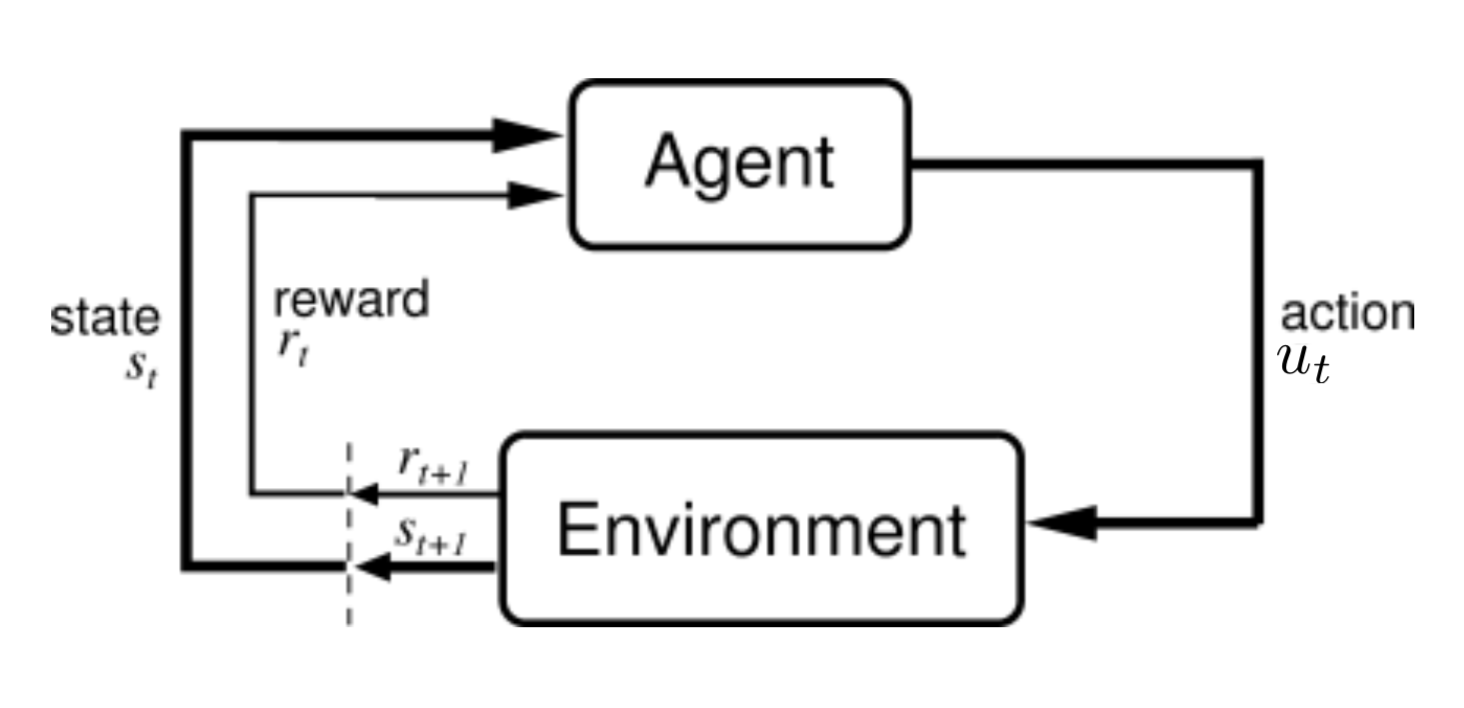
\includegraphics[scale=0.4] {images/rl_1.png}}
\caption{Basic Reinforcement Learning Setup (Figure courtesy \cite{SuttonBook})}
\label{fig:rl}
\end{figure}


\bigskip
\noindent
We wish to consider methods for learning the policy weights $\theta$ based on the gradient of some utility/performance measure $U(\theta)$) with respect to the policy weights. These methods seek to maximize performance, so their updates approximate gradient ascent in $U$. As is typical for gradient descent/ascent, 

\begin{flalign}
\boldsymbol{\theta}_{t+1} \coloneqq \boldsymbol{\theta}_t + \alpha \widehat{\nabla U(\boldsymbol{\theta}_t)}
\label{eqn:gd}
\end{flalign}

\bigskip
\noindent
where $\widehat{\nabla U(\boldsymbol{\theta}_t)}$ is a stochastic estimate whose expectation approximates the gradient of the performance measure $U$ with respect to its argument $\theta_t$. As we will see, $\widehat{\nabla U(\boldsymbol{\theta}_t)}$ will turn out to be something like $\nabla_{\theta} \mathbb{E}_{\tau}[R(\tau)]$, where $\tau$ is a \emph{trajectory} and $R(\tau)$ is the return for path $\tau$ (see Section \ref{sec:scorefunction}).




\section{Policy Optimization}
\label{sec:scorefunction}

In policy optimization we consider control policy $\pi_{\theta}$, the parameterized policy (parameterized by parameter vector $\theta$),
 and a utility/performance function $U(\theta)$, defined as follows:

\begin{flalign}
U(\theta) = \max_\theta \mathbb{E} \Bigg [\sum\limits_{t = 0}^{H - 1} R(s_t) | \pi_\theta \Bigg ]
\label{eqn:utility}
\end{flalign}

\bigskip
\noindent 
where $\pi_{\theta}(u | s)$ is a stochastic policy, that is, the probability of action $u$ in state $s$. Note that frequently the action is denoted by $a$, but we will
follow the notation of the control theory community and call the actions $u$. In addition, the utility (sometimes performance) function $U(\theta)$ is 
frequently referred to as $\eta(\theta)$ (for example, in \cite{Baxter:2001:IPE:1622845.1622855}); however we shall use $U(\theta)$ here.

\subsection{Why Policy Optimization?}
There are several reasons we might want to directly optimize our policy rather than say, a value function. These include

\begin{itemize}
\item Stochastic policies tend to smooth out the problem\footnote{Note that there are Deterministic Policy Gradient approaches,
 e.g. \cite{Silver:2014:DPG:3044805.3044850}.}
\item Policy optimization directly optimizes what we are interested in, namely $\pi_{\theta}(s,u)$
\item Frequently the policy $\pi$ is simpler that either value function Q or V
\item The state value function V does not prescribe actions, so would need a dynamics model (plus one or more Bellman backups)
\item Using the action-value function Q is problematic (difficult if not impossible) when the action space (the $u$'s) and or the state
spaces (the $s$'s) are continuous or high dimensional (such as in robotic arm manipulation). This is because instead of directly parameterizing a policy, 
Q-value learning methods estimate the Q-function as $Q_{\theta}(s, u)$. The greedy policy selects the (discrete) action maximizing value:
$u^{*}= \argmax\limits_{u} Q_{\theta}(s, u)$. Exploration can be performed using an $\epsilon$-greedy policy, which chooses a uniform random action with probability 
$\epsilon$ and otherwise uses the greedy action. By its off-policy nature, Q-learning permits repeated training use of samples. Note that on-policy TD(0) approaches 
such as SARSA \cite{SuttonBook} suffer from the same problem(s) since both SARSA and Q-learning use an $\epsilon$-greedy policy (i.e. $\max\limits_u Q(s,u)$ ) 
to strike the balance between exploration and exploitation.
\end{itemize}

\section{Likelihood Ratio Policy Gradients}

We want to compute the gradient $\nabla_{\theta} U(\theta)$ so that we can use gradient ascent/descent to improve the probability of good trajectories $\tau$ 
(Equation \ref{eqn:gd}). In this section we will derive the Likelihood Ratio Policy Gradient which we can use for this purpose.  Before doing so, however, first 
notice that Likelihood Ratio methods only change the probabilities of experienced paths, and further, these methods do not try to change the  actions taken in a given path. 

\bigskip
\noindent
Now, let $\tau$ denote a state-action sequence with \emph{horizon} $H$,  $s_0,u_0,\cdots,s_{H - 1},u_{H - 1}$ and let the total reward from 
trajectory $\tau$ be 

\bigskip
\begin{equation*}
R(\tau) = \sum\limits_{t = 0}^{H - 1} R(s_t,u_t)
\end{equation*}

\noindent
Notes:
\begin{itemize}
\item Note that $R(s_t,u_t)$ is a single rollout estimate of the action value function $Q(s_t,a_t)$
\item Lack of discounting (or $\gamma = 1$); we will add discounting later as a means to lower the variance of our estimator.
\end{itemize}

\bigskip
\noindent
Rewriting $U(\theta)$ we have

\bigskip
\begin{equation}
\label{eqn:u}
U(\theta) = \E_{\tau \sim P(\tau;\theta)} \Bigg [\sum\limits_{t = 0}^{H - 1} R(s_t,u_t) ; \pi_\theta \Bigg ] = \sum\limits_{\tau}P(\tau; \theta)R(\tau)
\end{equation}

\bigskip
\noindent
Here $H = |\tau |$ and $\tau$ is a trajectory (rollout) with $\tau = [s_0,u_0, s_1,u_1, \cdots s_{H-1},u_{H-1}]$.  

\bigskip
\noindent
Notes:
\begin{itemize}
\item State action pairs $[s_i,u_i]^{H-1}_{i = 0}$ in a trajectory $\tau$ are inconsistently numbered in the literature.  My guess:  In 
the Monte Carlo policy gradient estimator setting, $s_0$ is special and is dealt with in a kind of ad-hoc fashion.
\end{itemize}

\bigskip
\noindent
Given this notation/machinery, we can rewrite our goal as follows: Find $\theta$ such that 

\bigskip
\begin{equation}
\label{eqn:opt_u}
\max\limits_{\theta} U(\theta) = \max\limits_{\theta} \sum\limits_{\tau}P(\tau; \theta) R(\tau)
\end{equation}

\bigskip
\noindent
Because we want to solve our optimization problem (Equation \ref{eqn:opt_u}) using Stochastic Gradient Ascent (Equation \ref{eqn:gd}), 
we need to find the gradient of our performance function $U(\theta)$ with respect to its parameters $\theta$:

\bigskip
\begin{flalign}
\nabla_{\theta} U(\theta) &= \nabla_{\theta} \sum\limits_{\tau}P(\tau; \theta) R(\tau) \: \; \quad \qquad  \qquad \mathrel{\#} \text{definition of $U(\theta)$} \\
&= \sum\limits_{\tau} \nabla_{\theta} P(\tau; \theta) R(\tau) \; \;  \quad \qquad \qquad \mathrel{\#} \text{Leibniz integral rule: swap $\nabla$ and $\sum$} \\
\label{eqn:pit}
&= \sum\limits_{\tau} \frac{P(\tau;\theta)} {P(\tau;\theta)}  \nabla_{\theta} P(\tau; \theta) R(\tau) \; \: \qquad \mathrel{\#} \text{multiply by $1 =  \frac{P(\tau;\theta)} {P(\tau;\theta)}$} \\
&= \sum\limits_{\tau} P(\tau;\theta)  \frac{\nabla_{\theta} P(\tau; \theta)}{P(\tau;\theta)} R(\tau)  \: \; \qquad \mathrel{\#} \text{rearrange} \\
\label{eqn:log-dt}
&= \sum\limits_{\tau} P(\tau;\theta)  \nabla_{\theta} \log P(\tau; \theta) R(\tau) \; \quad \mathrel{\#} \frac{\nabla_{\theta} P(\tau;\theta)}{P(\tau;\theta)} = \nabla_{\theta} \log P(\tau;\theta) \\
&= \E_{\tau \sim P(\tau;\theta)} \Big [\nabla_{\theta} \log P(\tau; \theta) R(\tau) \Big ] \quad \mathrel{\#} \text{definition of expectation}
\label{eqn:expectation}
\end{flalign}

\bigskip
\noindent
Notes:
\begin{itemize}
\item Equation \ref{eqn:pit}: Multiplying by $\frac{P(\tau;\theta)} {P(\tau;\theta)}$ is sometimes called the "Probabilistic Identity Trick"  \cite{log_derivative_trick}. This allows us to form
the score function (see "Log Derivative Trick" in the next bullet). Ed: Not sure why these are called tricks.
\item Equation \ref{eqn:log-dt}:  $\frac{\nabla_{\theta} P(\tau;\theta)}{P(\tau;\theta)} = \nabla_{\theta} \log P(\tau;\theta)$ is known as the "Log Derivative Trick" \cite{log_derivative_trick} or 
sometimes the "likelihood ratio trick" or even the "REINFORCE trick" \cite{Williams1992} .
$\frac{\nabla_{\theta} p(x \mid \theta)}{p(x \mid \theta)}$ is called the "likelihood ratio" or "score function" in classical statistics. 
The log derivative trick is sometimes framed up like this: 
The gradient of something divided by something is the gradient of the log of something. Also frequently
pronounced "grad something divided by something is grad log something".
\item  Equation \ref{eqn:expectation}: This derivation reduces the computation of the gradient $\nabla_{\theta}U(\theta)$ to a simple expectation. 
This means, among other things,  that we know from the Strong Law of Larger Numbers (see Section \ref{sec:slln}) that an \emph{unbiased} estimate of the gradient $\hat{g}$
can be computed directly from our samples (Equation \ref{eqn:g-hat}).
\item Appendix A gives a slightly more general version of this derivation.
\end{itemize}

\bigskip
\noindent
So our result is that 

\begin{equation}
\nabla_{\theta} U(\theta) = \E_{\tau \sim P(\tau;\theta)} \Big [\nabla_{\theta} \log P(\tau; \theta) R(\tau) \Big ]
\label{eqn:egradient}
\end{equation}

\bigskip
\noindent
An immediate implication of the fact that the gradient is reduced to an expectation is that we can approximate the gradient ($\hat{g}$) with the empirical estimate for $m$ 
sample paths under policy $\pi_\theta$,  as follows:

\begin{equation}
\nabla_\theta U(\theta) \approx \hat{g} = \frac{1}{m} \sum\limits_{i = 1}^{m} \nabla_{\theta} \log  P(\tau^{(i)} ; \theta) R(\tau^{(i)})
\label{eqn:g-hat}
\end{equation}

\bigskip
\noindent
A couple of notes here. First, we know by the law of large numbers (Appendix B) that 
$\frac{1}{m} \sum\limits_{i = 1}^{m} \nabla_{\theta} \log  P(\tau^{(i)} ; \theta) R(\tau^{(i)}) \rightarrow \nabla_\theta U(\theta)$ with probability one; this is
another way of saying our estimator $\hat{g}$  is unbiased. Next,  the estimate $\hat{g}$ holds even if 

\begin{itemize}
\item $R(\tau)$ is not continuous and/or unknown
\item The sample space of paths is a discrete set
\end{itemize}

\bigskip
\noindent
So for each sample path we need to be able to compute $\nabla_{\theta} \log  P(\tau^{(i)};\theta)$. How might we do this? We can decompose $P(\tau^{(i)}; \theta)$ into 
a states and actions, as follows:

\begin{flalign}
\nabla_{\theta} \log P(\tau^{(i)}; \theta) &= \nabla_{\theta} \log \Bigg [ \prod\limits_{t = 0}^{H - 1} \underbrace{P(s^{(i)}_{t+1} | s^{(i)}_t, u^{(i)}_t)}_{\text{dynamics/plant model}} \cdot 
\underbrace{\pi_{\theta}(u^{(i)}_t |  s^{(i)}_t)}_{\text{policy}} \Bigg ]  \\
\label{eqn:log_prod}
&= \nabla_{\theta} \Bigg [\sum\limits_{i = 0}^{H - 1} \log P(s^{(i)}_{t+1} | s^{(i)}_t, u^{(i)}_t) + \sum\limits_{i = 0}^{H - 1} \log \pi_{\theta}(u^{(i)}_t |  s^{(i)}_t) \Bigg ]  \\
&= \nabla_{\theta} \sum\limits_{i = 0}^{H - 1} \log P(s^{(i)}_{t+1} | s^{(i)}_t, u^{(i)}_t)  + \nabla_{\theta} \sum\limits_{i = 0}^{H - 1} \log \pi_{\theta}(u^{(i)}_t |  s^{(i)}_t) \\
\label{eqn:dynamics_model}
&= \sum\limits_{i = 0}^{H - 1} \nabla_{\theta}  \log P(s^{(i)}_{t+1} | s^{(i)}_t, u^{(i)}_t)  + \sum\limits_{i = 0}^{H - 1} \nabla_{\theta}  \log \pi_{\theta}(u^{(i)}_t |  s^{(i)}_t) \\
\label{eqn:ldt}
&= \sum\limits_{i = 0}^{H - 1} \nabla_{\theta}  \log \pi_{\theta}(u^{(i)}_t |  s^{(i)}_t)  
\end{flalign}

\bigskip
\noindent
So $\nabla_{\theta} \log P(\tau^{(i)}; \theta) = \sum\limits_{i = 0}^{H - 1}  \nabla_{\theta} \log \pi_{\theta}(u^{(i)}_t |  s^{(i)}_t)$. This result is stated
in a slightly different form in Baxter \& Bartlett \cite{Baxter:2001:IPE:1622845.1622855}:

\begin{flalign}
\frac{\nabla_{\theta} P(\tau^{(i)}; \theta)}{P(\tau^{(i)}; \theta)} = 
\sum\limits_{i = 0}^{H - 1} \frac{\nabla_{\theta} \pi_{\theta}(u^{(i)}_t |  s^{(i)}_t)}{ \pi_{\theta}(u^{(i)}_t |  s^{(i)}_t)}
\end{flalign}

\bigskip
\noindent
You can see that this is equivalent to Equation \ref{eqn:ldt} by applying the "log derivative trick" \cite{log_derivative_trick},  $\nabla \log f(X)= \frac{\nabla f(X)}{f(X)}$,
to both sides of Equation \ref{eqn:ldt}.

\bigskip
\noindent
Notice that the dynamics/plant model $P(s^{(i)}_{t+1} | s^{(i)}_t, u^{(i)}_t)$  drops out of Equation \ref{eqn:dynamics_model}. This is because the 
dynamics of the system do not depend on the parameters $\theta$ of our model, so the gradient is zero. This is a handy result as we are trying 
to do model-free learning (model-based learning would require the dynamics as part of the model).  Now we can compute an unbiased 
estimate\footnote{Unbiased means that $\E[\hat{g}] = \nabla_{\theta}U(\theta)$.} 
of the gradient without the need for a dynamics model:

\begin{flalign}
\hat{g} & = \frac{1}{m} \sum\limits_{i = 1}^{m} \nabla_{\theta} \log P(\tau^{(i)};\theta) R(\tau^{(i)})
\label{eqn:g-hat-1}
\end{flalign}

\noindent
where 

\begin{flalign}
\nabla_{\theta} \log P(\tau^{(i)};\theta)  = \sum\limits_{t = 0}^{H - 1} \nabla_{\theta} \log \pi_{\theta} (u^{(i)}_t  | s^{(i)}_t)
\label{eqn:likelihood_ratio}
\end{flalign}

\bigskip
\noindent
Note that the gradients $\nabla_{\theta} \log \pi_{\theta} (u^{(i)}_t  | s^{(i)}_t)$ required by Equation \ref{eqn:likelihood_ratio} are exactly what are computed by
the backpropagation algorithm on the (log) policy neural network.

\bigskip
\noindent
Combining Equations \ref{eqn:g-hat-1} and \ref{eqn:likelihood_ratio} gives

\begin{flalign}
\hat{g} & = \frac{1}{m} \sum\limits_{i = 1}^{m} \sum\limits_{t = 0}^{H - 1} \nabla_{\theta} \log \pi_{\theta} (u^{(i)}_t  | s^{(i)}_t) R(\tau^{(i)})
\label{eqn:combined-g-hat}
\end{flalign}

\bigskip
\noindent

Equation \ref{eqn:combined-g-hat} is our estimate of the gradient $g = \nabla_{\theta} U(\theta)$, where

\begin{flalign}
g & =  \E_{\tau \sim P(\tau;\theta)} \Big [\nabla_{\theta} \log P(\tau; \theta) R(\tau) \Big ] \\
&= \E_{s_{t}, u_t \sim P(\tau; \theta)}  \Bigg [\sum\limits_{t = 0}^{H-1} \nabla_{\theta} \log \pi_{\theta} (u_t  | s_t) \phi(s_t) \Bigg ]
\label{eqn:combined-g}
\end{flalign}

\bigskip
\noindent
Here $s_0 \sim \rho(s_0)$ is a distribution over initial states and $\phi(s_t) = R(u_t, s_t)$; we will explore the tradeoff 
between variance and bias for different options for $\phi_t$ below.

\bigskip
\noindent
We can also relax the "episodic" assumption (changing the inner sum from $t = 0 $ to $H -1$ into a sum from $t = 0$ to $\infty$ 
in Equation \ref{eqn:combined-g-hat}) by using a \emph{discount factor} $\gamma \in [0,1]$; as we will see below that we can use $\gamma$ 
to reason about the termination  of $\hat{g}$. 

\section{Reducing the Variance of the (Gradient) Estimator}
\label{sec:variance}
The likelihood ratio estimate of the policy gradient as described so far can be very sample inefficient due to its high variance. The next few sections describe straight forward ways to 
reduce the variance of the estimator $\hat{g}$. The methods described below are part of a more general approach to variance reduction which uses one ore more \emph{control variates} 
\cite{szechtman2003}:
\begin{itemize}
\item Centering our estimate around a constant baseline \cite{Williams1992}. As we shall see (Section \ref{sec:baseline}, baselines effectively account for and remove the effects of past actions.
\item Taking advantage of temporal structure based on the observation that future actions do not depend on past rewards (unless the policy has been changed) . This can result in a significant 
reduction of the variance of the policy gradient estimate. See Section II. B (1) of \cite{Peters:2006fk}.
\item Use an estimate of the state value function, $V^{\pi}(s^{(i)}_t)$ as a control variate. The value function is a typical control variate used
with Monte Carlo estimators \cite{Greensmith:2004:VRT:1005332.1044710}.  See for example Equation \ref{eqn:a2c}.
\item More advanced Policy Gradient methods such as Trust Region Policy Optimization \cite{DBLP:journals/corr/SchulmanLMJA15} and Proximal Policy Optimization Algorithms \cite{2017arXiv170706347S} 
provide still better estimates. These ideas relate to the one of the main reasons for their use in robotics: how to make "small" changes to the policy $\pi_\theta$ while improving it.  
Section II C \cite{Peters:2006fk} discusses this point in some detail. 
\end{itemize}

\subsection{Aside on Control Variates}
\label{sec:control_variates}
Suppose we wish to estimate $\mu = \E[f]$ where we know that $f$ has high variance (such as is the case for Monte Carlo gradient estimators). 
The control variate method is to find a function $g$, the control variate, which without loss of generality has $\E[g] = 0$. Then

\begin{flalign*}
\mu = \E[f] = \E[f - g] \approx \frac{1}{n}\sum\limits_{i= 1}^{n} \Big [ f(x_i) - g(x_i) \Big ] 
\end{flalign*}

\bigskip
\noindent
If we can choose $g$ such that  $\sigma^{2}_{(f -  g)}$ is small, then we will have found a way to reduce the variance of our original estimator.
This means that we want to find an identity $\E[g] = 0$ for a large class of functionals $g$ so that we will have flexibility in choosing $g$. 
The  identity typically used in the Policy Gradient setting is 

\begin{flalign}
\E_{s \sim P(s), u \sim \pi_{\theta} (u | s)} \Big [ \nabla_{\theta} \log \pi_{\theta}(u | s) \phi (s) \Big ] = 0
\label{eqn:ident}
\end{flalign}

\bigskip
\noindent
where $\phi(s)$ is the control variate. You can see this pretty easily:

\begin{flalign*}
\E_{s, u} \Big [ \nabla_{\theta} \log \pi_{\theta}(u | s) \phi (s) \Big ] 
&= \E_{s} \Bigg [ \E_{u} \Big [ \nabla_{\theta} \log \pi_{\theta}(u | s) \phi (s) \Big ] \Bigg ]
\: \; \qquad  \qquad
\mathrel{\#} \text{def expectation} \\
&= \E_{s} \Bigg [ \phi (s) \cdot \E_{u} \Big [ \nabla_{\theta} \log \pi_{\theta}(u | s)  \Big ] \Bigg ]
\qquad \qquad
\mathrel{\#} \phi(s) \text{ doesn't depend on } u\\
&= \E_{s} \big [ \phi (s) \cdot 0 \big ]
\qquad \qquad \qquad \qquad \qquad \qquad 
\mathrel{\#} \E \big [\nabla_{\theta} \log \pi(u | s) \big ] = 0  \\
&= \E_{s} \big [ 0 \big ] \\
&= 0
\end{flalign*}

\bigskip
\noindent
We can also see pretty easily that $\E \big [\nabla_{\theta} \log \pi(u | s) \big ] = 0$. More generally

\begin{flalign}
\label{eqn:score-fn}
\E_{x \sim p_{\theta} (x)}\big [\nabla_{\theta} \log p_{\theta}(x) \big] & = \int p_{\theta}(x) \nabla_{\theta} \log p_{\theta}(x) dx   \quad \mathrel{\#} \text{def expectation} \\
&= \int \frac{\nabla_\theta p_\theta(x)}{p_\theta(x)} p_\theta(x) dx  \; \; \qquad \mathrel{\#} \nabla_{\theta} \log p_{\theta}(x)  
= \frac{\nabla_{\theta} p_\theta(x)}{p_\theta(x)} \\
&= \int \frac{p_\theta(x)}{p_\theta(x)} \nabla_\theta p_\theta(x) dx  
\; \; \qquad \mathrel{\#} \text{rearrange}\\
&= \int \nabla_\theta p_\theta(x) dx  \qquad  \quad \qquad \mathrel{\#} \frac{p_\theta(x)}{p_\theta(x)} = 1 \\
&= \nabla_\theta \int p_\theta(x) dx  \;\;\;  \qquad \qquad \mathrel{\#} \text{swap $\int$ and $\nabla$} \\
&= \nabla_{\theta} 1 \quad  \qquad \qquad  \qquad \qquad \mathrel{\#}  \int_x p_\theta(x) dx = 1  \text{ ($p$ a density)}\\
&= 0  \; \quad  \quad \qquad \qquad \qquad \qquad \mathrel{\#} \text{for c any constant } \nabla c = 0
\end{flalign}

\bigskip
\noindent
There are several options for $\phi(s_t)$ \cite{2015arXiv150602438S}. As we will see, these include (abusing notation slightly):

\begin{flalign*}
\phi(s_t) &= \sum\limits_{t = 0}^{H - 1} r_t
\: \;  \qquad \qquad \qquad \qquad \qquad
\mathrel{\#} \text{total reward of the trajectory } \tau \\
\phi(s_t) &= \sum\limits_{t' = t}^{H - 1} r_t
\; \; \qquad \qquad \qquad \qquad \qquad 
\mathrel{\#} \text{total reward following action $u_t$} \\
\phi(s_t) &= \sum\limits_{t' = t}^{H - 1}  r_t -b(s_t) 
\, \; \quad \qquad \qquad \qquad 
\mathrel{\#} \text{baselined version of previous expression} \\
\phi(s_t) &= r_t +V^{\pi}(s_{t+1}) - V^{\pi, \gamma}(s_t)
\; \; \qquad
\mathrel{\#} \text{TD residual, denoted } \delta^V_t( s_{t+1})\\
\phi(s_t, u_t) &= Q^{\pi} (s_{t}, u_{t})
\quad \qquad \qquad \qquad \qquad
\mathrel{\#} \text{state-action value function} \\
\phi(s_t, u_t) &= A^{\pi} (s_{t}, u_{t})
\quad \qquad \qquad \qquad \qquad
\mathrel{\#} \text{advantage function: }  A^{\pi} (s_{t}, u_{t}) =  Q^{\pi} (s_{t}, u_{t}) -  V^{\pi}(s_t)\\
\end{flalign*}

\bigskip
\noindent
where $r_t  \sim P(r_t \mid s_t,u_t)$ is the probability of reward $r_t$ when taking action $u_t$ in state $s_t$, and 
\begin{flalign*}
V^{\pi}(s_t) &= \E_{s_{t+1} \sim p(s_{t+1} | s_t, u_t), u_t \sim \pi(u_t|s_t)}\Bigg [ \sum\limits_{l = 0}^{H - 1}  r_{t+l} \Bigg ] 
\, \quad \qquad  \qquad 
\mathrel{\#} \text{finite horizon state value function} \\
Q^{\pi}(s_t,u_t) &= \E_{s_{t+1} \sim p(s_{t+1} | s_t, u_t), u_{t+1} \sim \pi(u_{t+1} | s_{t+1})} \Bigg [ \sum\limits_{l = 0}^{H - 1} r_{t+l} \Bigg ] 
\; \;  \qquad 
\mathrel{\#} \text{finite horizon state-action value function} \\
A^{\pi}(s_t,u_t) &= Q^{\pi}(s_t,u_t) - V^{\pi}(s_t) 
\; \;  \; \; \qquad \qquad \qquad \qquad \qquad \qquad 
\mathrel{\#} \text{finite horizon advantage function}
\end{flalign*}


\bigskip
\noindent
Notes:
\begin{itemize}
\item if $\phi (\cdot)$ depends on $u$ (e.g., $\phi(s_t,u_t)) = A^{\pi}(s_t,u_t)$) the estimator will typically be biased
\item Recall that an estimator $\hat{g}$ is \emph{unbiased} if $\E[\hat{g}] = g$
\end{itemize}

\bigskip
\noindent
Interestingly, $\E_{s,u} \big [A^{\pi}(s,u) \nabla \log \pi(u|s) \big] = E_{s,u} \big [Q^{\pi}(s,u) \nabla \log \pi(u|s) \big]$. Here's one 
way to see this:

\begin{flalign*}
\E_{s,u} \big [A^{\pi}(s,u) \nabla \log \pi(u|s) \big] &= \E_{s,u} \big [ (Q^{\pi}(s,u) - V^{\pi}(s))  \nabla \log \pi(u|s)  \big] \\
&= \E_{s} \Big [ \E_{u} \big [  \big ( Q^{\pi}(s,u) - V^{\pi}(s) \big )  \nabla \log \pi(u|s)  \big] \Big ] \\
&= \E_{s} \Big [ \E_{u} \big [   Q^{\pi}(s,u) \nabla \log \pi(u|s) - V^{\pi}(s) \nabla \log \pi(u|s)    \big] \Big ] \\
&= \E_{s} \Big [ \E_{u} \big [  Q^{\pi}(s,u) \nabla \log \pi(u|s)   \big ] - \E_{u} \big [ V^{\pi}(s) \nabla \log \pi(u|s) \big ] \Big ] \\
&= \E_{s} \Big [ \E_{u} \big [  Q^{\pi}(s,u) \nabla \log \pi(u|s) \big ] - V^{\pi}(s)  \cdot \E_{u} \big [  \nabla \log \pi(u|s)  \big ] \Big ] \\
&= \E_{s} \Big [ \E_{u} \big [  Q^{\pi}(s,u) \nabla \log \pi(u|s) \big ] - V^{\pi}(s)  \cdot 0 \Big ] \\
&= \E_{s} \Big [ \E_{u} \big [  Q^{\pi}(s,u) \nabla \log \pi(u|s) \big ] \Big ] \\
&= \E_{s,u} \Big [  Q^{\pi}(s,u) \nabla \log \pi(u|s) \Big ] 
\end{flalign*}

\bigskip
\noindent
The key step here is that in the term $\E_{u} \big [ V^{\pi}(s) \nabla \log \pi(u|s) \big ]$, $V^{\pi}(s)$ doesn't depend on $u$, so we
can factor it out of the expectation. This leaves us with the term $V^{\pi}(s) \cdot \E_{u} \big [  \nabla \log \pi(u|s)  \big ]$ and we know
that by Equation \ref{eqn:score-fn} $\E_{u} \big [  \nabla \log \pi(u|s)  \big ] = 0$. So the whole term is zero.\footnote{Sorry there wasn't 
enough space to write comments in-line.}

\bigskip
\noindent
As mentioned above (and I'll just note here),  one weakness with the identity given in Equation \ref{eqn:ident} (and hence Equation \ref{eqn:pgt}) 
is that $\phi(s)$ can not depend on the action $u$. Q-Prop \cite{2016arXiv161102247G}, approaches based on Stein's Identity \cite{2017arXiv171011198L}, and
Action-Dependent Factorized Baselines \cite{2018arXiv180307246W} for example, overcome this limitation by introducing action-dependent baseline functions.
However, recent work questions the effectiveness of action-dependent baselines \cite{2018arXiv180210031T}.

\bigskip
\noindent
If we combine Equation \ref{eqn:ident} with the Policy Gradient Theorem \cite{Sutton:1999:PGM:3009657.3009806} we get

\begin{flalign}
\label{eqn:pgt}
\nabla J(\theta) = \E_{u \sim \pi_{\theta} (u | s)} \Big [ \nabla_{\theta} \log \pi_{\theta}(u | s) \big ( Q^{\pi} (s,t) - \phi (s) \big ) \Big ]
\end{flalign}

\bigskip
\noindent
which generalizes quite a few policy gradient algorithms including REINFORCE \cite{Williams1992}, where $\phi(s) = b$ ($b$  
is an empirically determined constant baseline function),  and Advantage Actor-Critic (A2C) \cite{SuttonBook}, where $\phi(s) = V^{\pi}(s)$
($V^{\pi}(s)$ is a state-dependent baseline function). We'll see more detail on all of this below.


\bigskip
\noindent
To fill in some detail and see how this all works, consider a Monte Carlo approximation of $\E[X]$ 


\begin{equation}
\E[X] \approx \overline{X}(n) = \frac{1}{n} \sum\limits_{i = 1}^{n} X_i
\end{equation}

\bigskip
\noindent
where the $n$ samples from $p(X)$ are independent and identically distributed (iid)\footnote{$p(X)$ is the (unknown) Data Generating Distribution.}.
Now,  let $C$ be any other random variable over the same space as $X$ with known mean $\E[C]$ 
and let $b$ be some constant. Then consider the random variable $Y$ given by

\begin{equation}
\label{eqn:y}
Y = X - b (C - \E[C])
\end{equation}


\bigskip
\noindent
Here we can think of $Y$ a "corrected" or controlled estimator of $\E[Y]$ where the deviations of $C_i$'s  
from their known means $\E[C_i]$ are used to correct  samples of $X$,  drawing the $X_i$'s  closer to $\E[X]$ and hence reducing the variance
of the  estimator. Here information about the $C_i$'s and their means is being \emph{extracted} and \emph{transferred} to our estimate 
of $\E[X]$, hopefully reducing the variance.


\bigskip
\noindent
This method of introducing a random variable $C$ for purposes of reducing variance of another random variable (in this case $X$) is called
the control variates method, and $C - \E[C]$ is frequently called the control variate for estimating $\E[X]$. 


\bigskip
\noindent
Note that among other properties,  $Y$ has the same mean as $X$, than is, $\E[Y] = \E[X]$. To see this, notice that

\begin{flalign}
\E[Y] &= \E[X - b (C - \E[C])]
\:  \qquad \qquad \qquad
 \mathrel{\#} \text{Expected value of $Y$ (Equation \ref{eqn:y})} \\
 &= \E[X] - \E[b (C - \E[C]]
 \: \: \quad \qquad \qquad 
 \mathrel{\#} \E[X - Y] = \E[X] - \E[Y]  \\
 &= \E[X] - b\E[ (C - \E[C]]
 \; \quad \qquad \qquad
 \mathrel{\#} \E[bX] = b\E[X] \\
 &= \E[X] - b \big (\E[C] - \E[\E[C]] \big )
 \; \; \quad \quad \quad
 \mathrel{\#} \E[X - Y] = \E[X] - \E[Y] \\
 &= \E[X] - b \big (\E[C] - \E[C] \big )
 \; \; \; \quad \quad \qquad
 \mathrel{\#} \E[\E[X]]  = \E[X] \; (\E[X] \text{ is a constant}) \\
 &= \E[X] - b \cdot 0  
 \; \; \;   \quad  \qquad \qquad \qquad \qquad
 \mathrel{\#} f(X) - f(X) = 0   \\
 &= \E[X]
\; \; \; \qquad \qquad \qquad \qquad \qquad \qquad
 \mathrel{\#} \E[Y]  = \E[X] 
 \end{flalign}


\bigskip
\noindent
This is handy since if we could simulate iid instances of $Y,$ $\{Y_i\}^{n}_{i = 1}$, then we could use  $\overline{Y} (n)$ as our estimator
instead of $\overline{X}(n)$. The reason we would like to use $\overline{Y} (n)$  rather than $\overline{X} (n)$ is that, in addition
to $X$ and $Y$ having the same mean, we can use the basic properties of variance\footnote{In particular,  $\sigma^{2}_{(X - Y)} = \sigma^2_{X} + \sigma^2_{Y} - 2 \sigma^2_{X,C}$.} 
to see how to directly reduce the variance of $\overline{Y} (n)$. To see this, first note that 

\begin{equation}
\label{eqn:var_y}
\sigma^{2}_{Y} = \sigma^{2}_{X} + b^2 \sigma^{2}_{C} - 2b \sigma^2_{X,C}
\end{equation}

\bigskip
\noindent
where $\sigma^2_{X,C}$ is the \emph{covariance}\footnote{$\sigma^2_{X,C}$ and  $\Cov(X,C)$  seem to be used interchangeably
in the literature.} between $X$ and $C$.

\bigskip
\noindent
Rearranging Equation \ref{eqn:var_y} a bit we see that 

\begin{equation}
\sigma^{2}_{Y}  = \sigma^{2}_{X} - b  \big (2 \sigma^2_{X,C} - b \sigma^{2}_{C} \big )
\end{equation}

\bigskip
\noindent
So  $\overline{Y}(n)$ can have lower variance than $\overline{X}(n)$ if we can manage 
to choose $b$ and $C$ such that  $2 \sigma^2_{X,C} - b \sigma^{2}_{C} > 0$, that is, 
$\sigma^2_{X,C} > \frac{b}{2} \sigma^{2}_{C}$. Said another way, our new estimator 
$\overline{Y}(n)$ can have lower variance than $\overline{X}(n)$
whenever $\sigma^2_{X,C} > \frac{b}{2} \sigma^{2}_{C}$. 
The covariance between $X$ and $C$, $\sigma^2_{X,C}$, can be thought of as the information that $C$ contains about $X$.

\bigskip
\noindent
For a given $C$, we can view Equation \ref{eqn:var_y} as a function of $b$, namely $g(b) = \sigma^{2}_{Y} (b)$, 
and then using a bit of calculus we see that

 \begin{flalign}
 \frac{\partial g(b)}{\partial b} &= \frac{\partial}{\partial b} \big ( \sigma^{2}_{X} + b^2 \sigma^{2}_{C} - 2b \sigma^2_{X,C} \big ) 
  \: \; \; \quad \qquad
 \mathrel{\#} \text{definition of $g(b)$, Equation \ref{eqn:var_y}} \\
 &= \frac{\partial}{\partial b} \sigma^{2}_{X} + \frac{\partial}{\partial b}  b^2 \sigma^{2}_{C} - \frac{\partial}{\partial b}  2b \sigma^2_{X,C} 
\: \qquad
 \mathrel{\#} \frac{\partial (f+ g)}{\partial \theta} =  \frac{\partial f}{\partial \theta}  + \frac{\partial g}{\partial \theta} \\
 &= \frac{\partial}{\partial b}  b^2 \sigma^{2}_{C} - \frac{\partial}{\partial b}  2b \sigma^2_{X,C} 
\quad  \qquad \quad \qquad
 \mathrel{\#} \sigma^2_{X} \text{ doesn't depend on } b \text{ so } \frac{\partial}{\partial b} \sigma^{2}_{X} = 0\\
 &= 2b \sigma^2_C  - \frac{\partial}{\partial b}  2b \sigma^2_{X,C} 
 \; \quad \qquad \qquad \qquad
 \mathrel{\#}  \text{power rule: }  \frac{\partial}{\partial x} x^n = nx^{n-1}  \\
 &= 2b \sigma^2_C  - 2\sigma^2_{X,C} 
\quad  \qquad \qquad \qquad \qquad
\mathrel{\#} \text{power rule again}
\end{flalign}


\bigskip
\noindent
To find $b^*$,  the minimum value of $b$,  set $\frac{\partial g(b)}{\partial b} =  2b \sigma^2_C  - 2\sigma^2_{X,C} = 0$ 
and solve for $b$. This yields:

 \begin{flalign}
 b^* &= \frac{\sigma^2_{X,C}}{ \sigma^{2}_{C}} 
 \end{flalign}

\bigskip
\noindent
The variance of $b^*$, $\sigma^{2}_{Y} (b^*)$,  is then defined as follows:

 \begin{flalign}
 \sigma^{2}_{Y} (b^*) &= \sigma^{2}_{X} (1- \rho^2_{X,C})
 \end{flalign}

\bigskip
\noindent
where the \emph{correlation coefficient} $\rho_{X,C} = \sigma^2_{X,C}/\sigma_{X} \sigma_{C}$. Thus by choosing any $C$ for which $\sigma^2_{X,C} \neq 0$
we can always reduce the variance of the estimator. 

\bigskip
\noindent
All good but in practice we likely won't be able to compute the value of $b^*$  since it is unlikely that we would know $\sigma^2_{X,C}$ and we might not even know $\sigma^{2}_{C}$.
However,  we could estimate $b^*$  in advance by simulation:  Choose a large $n$ and estimate $b^*$ as follows:

 \begin{flalign*}
b^* \approx  b^*(n) = \frac{\sum\limits_{i = 1}^{n} (X_i - \overline{X}(n))  (C_i - \E[C])}
{\sum\limits_{i = 1}^{n} (C_i - \E[C])^2}
 \end{flalign*}

\bigskip
\noindent
Said another way,  first run one simulation with large $n$ to obtain the estimate $b^*(n)$, and then use that fixed value throughout our desired Monte Carlo simulation.

\bigskip
\noindent
An effective control variate for $X$, say $Y$, needs to satisfy two requirements (to simplify the discussion we consider a scalar control):
\begin{enumerate}
\item $X$ and $Y$ need to be correlated\footnote{That is, $\sigma^2_{X,Y} \neq 0$.}. That is,  $Y$ must carry some information about $X$.
\item  $\E[Y]$ needs to be known
\end{enumerate}


\bigskip
\noindent
As mentioned ablve, the use of different control variates yield different variance reduction methods. 
Examples from Reinforcement Learning include REINFORCE \cite{Williams1992}, where a constant baseline function is chosen as a control variate. 
Advantage Actor-Critic (A2C) \cite{SuttonBook} uses a state-dependent baseline function as the control variate, which is often set to be an estimation 
of the state-value function $V^\pi(s) = \E_{a \sim \pi(a|s)} [Q^{\pi}(s,a)]$ so that $\hat{Q}^{\pi}(s,a) - \hat{V}^{\pi}(s)$ is an estimator of the advantage
function $A$.  Q-prop \cite{2016arXiv161102247G} proposes a more general baseline function that linearly depends on the actions. 
\cite{2017arXiv171011198L} extends the control variate methods used in REINFORCE and A2C by introducing more general action-dependent 
baseline functions based on Stein's Identity.

\bigskip
\noindent
In summary, the basic idea behind the control variate method is to subtract some baseline function which has (analytically) zero expectation from a 
Monte Carlo gradient estimator.  It is pretty easy to show that the resultant estimator does not in theory introduce additional bias (see Equation \ref{eqn:g-hat+baseline})  
but can have significantly lower variance. The reduction in variance becomes possible when the control variate is chosen so that its variance effectively cancels out 
the variance of the original gradient estimator. 

\subsection{Using a (constant) Baseline}
\label{sec:baseline}

This idea seems to have originated in Williams \cite{Williams1992}. To see how adding a baseline can reduce the variance of our estimator, recall that the gradient estimator $\hat{g}$ is defined as follows:

\begin{equation}
\nabla_\theta U(\theta) \approx \hat{g} = \frac{1}{m} \sum\limits_{i = 1}^{m} \nabla_{\theta} \log  P(\tau^{(i)} ; \theta) R(\tau^{(i)})
\end{equation}

\bigskip
\noindent
We can add a baseline $b$ to capture the idea that what we really care about is how good the reward $R(t)$ is compared to some baseline, such as the mean reward. 
The way we might formalize this is as follows:

\begin{equation}
\nabla_\theta U(\theta) \approx \hat{g} = \frac{1}{m} \sum\limits_{i = 1}^{m} \nabla_{\theta} \log  P(\tau^{(i)} ; \theta) (R(\tau^{(i)})  b)
% \label{eqn:g-hat}
\end{equation}

\bigskip
\noindent
$b$ here is assumed to be constant, but in reality as long as $b$ doesn't depend on the action $u$, adding a baseline $b$ does not introduce bias to the gradient estimate 
$\hat{g}$ \cite{Williams1992}. Why? We can see this pretty easily. The following result is used in Equation 7 of  
\cite{Peters:2006fk}; there they state that $\int_{\mathbb{T}} \nabla_{\theta} p_{\theta}(\tau) \; d\tau = 0$, which is important as
can be seen (with a bit more detail) in Equations \ref{eqn:before_sum_zero} through \ref{eqn:sum_zero} of the following:

\begin{flalign}
\label{eqn:g-hat+baseline}
\E[\hat{g}] &= \E_{\tau \sim P(\tau;\theta)} \Big [\nabla_{\theta} \log P(\tau; \theta) [R(\tau) - b] \Big ] 
 \; \; \; \quad \qquad
 \mathrel{\#} \text{definition of } \hat{g} \\
&= \sum\limits_{\tau} P(\tau;\theta)  \nabla_{\theta} \log P(\tau; \theta) [R(\tau) - b]  
\, \quad \quad \qquad
 \mathrel{\#} \text{definition of  expectation}\\
&=  \sum\limits_{\tau}   \nabla_{\theta} P(\tau; \theta) [R(\tau)  -  b]  
\; \; \; \qquad \qquad \qquad \qquad
 \mathrel{\#} \frac{\nabla_{\theta} P(\tau;\theta)}{P(\tau;\theta)} = \nabla_{\theta} \log P(\tau;\theta) \\
&=  \sum\limits_{\tau} \Big [\nabla_{\theta} P(\tau; \theta) R(\tau) -  b \cdot \nabla_{\theta} P(\tau; \theta) \Big ] 
\: \: \quad \quad \quad
 \mathrel{\#} \text{multiply through} \\
&=  \sum\limits_{\tau}  \nabla_{\theta} P(\tau; \theta) R(\tau)  - \; \sum\limits_{\tau} b \cdot \nabla_{\theta} P(\tau; \theta)
\, \; \quad \quad
 \mathrel{\#} \text{distribute $\sum$} \\
\label{eqn:before_sum_zero}
&=  \sum\limits_{\tau}  \nabla_{\theta} P(\tau; \theta) R(\tau) -  b \cdot \sum\limits_{\tau} \nabla_{\theta} P(\tau; \theta)
\: \; \; \quad \quad
 \mathrel{\#} \text{factor out $b$} \\
&=  \sum\limits_{\tau}  \nabla_{\theta} P(\tau; \theta) R(\tau -  b \cdot  \nabla_{\theta} \sum\limits_{\tau} P(\tau; \theta)
\qquad \quad
 \mathrel{\#} \text{swap } \sum\limits_{\tau} \text{ and } \nabla_\theta \\
&=  \sum\limits_{\tau}  \nabla_{\theta} P(\tau; \theta) R(\tau)  -  b \cdot  \nabla_{\theta} 1
\quad \qquad \qquad \qquad
 \mathrel{\#} \sum\limits_{\tau} P(\tau; \theta) = 1 \\
\label{eqn:sum_zero}
&=  \sum\limits_{\tau}  \nabla_{\theta} P(\tau; \theta) R(\tau) -  b \cdot 0
\; \qquad \qquad \qquad \qquad
 \mathrel{\#} \nabla c = 0 \text{ for constant $c$} \\
&=  \sum\limits_{\tau}  \nabla_{\theta} P(\tau; \theta) R(\tau) 
\; \quad \qquad \qquad \qquad \qquad \qquad
 \mathrel{\#} b \cdot 0 = 0 \\
&= \nabla_{\theta} U(\theta) 
\qquad \qquad \qquad \qquad \qquad \qquad \qquad \qquad
\mathrel{\#} \sum\limits_{\tau}  \nabla_{\theta} P(\tau; \theta) R(\tau)  =  \nabla_{\theta} U(\theta) 
\end{flalign}

\bigskip
\noindent
So $\E[\hat{g} ] = \nabla_{\theta} U(\theta)$, that is,  $\hat{g}$ is unbiased, even if we subtract an arbitrary baseline $b$ (so long as 
$b$ doesn't depend on the action $u$).  

\subsection{Exploiting Temporal Structure}
 We know that in general, removing terms that don't depend on the current action can reduce variance.  
 We can take advantage of this observation and of temporal structure of our problem.
In particular, we know that future actions do not depend on past rewards (unless the policy has been changed). So if we can remove past rewards 
from our current estimate $\hat{g}$, we would expect a significant reduction of the variance of our gradient estimate (which in general we observe).  
This observation seems to have originated in Williams \cite{Williams1992}. See also Section II. B (1) of \cite{Peters:2006fk}.
We can implement this strategy in our current estimate $\hat{g}$ by simply removing rewards received at times $j < t -1$, where 
$t$ is the current timestep in the current rollout $i$, as follows:

\begin{flalign}
\hat{g} &= \frac{1}{m} \sum\limits_{i = 1}^{m} \nabla_{\theta} \log P(\tau^{(i)}; \theta) (R(\tau^{(i)}) - b) \\
&= \frac{1}{m} \sum\limits_{i = 1}^{m} \Bigg ( \sum\limits_{t = 0}^{H - 1} \nabla_{\theta} \log \pi_{\theta} (u^{(i)}_t | s^{(i)}_t) \Bigg )
\Bigg (\sum\limits_{t = 0}^{H - 1} R(s^{(i)}_t, u^{(i)}_t) -b\Bigg ) \\
\label{eqn:t=0}
&= \frac{1}{m} \sum\limits_{i = 1}^{m} \Bigg ( \sum\limits_{t = 0}^{H - 1} \nabla_{\theta} \log \pi_{\theta} (u^{(i)}_t | s^{(i)}_t) \Bigg [
\Bigg (\sum\limits_{j = 0}^{t - 1} R(s^{(i)}_j, u^{(i)}_j) \Bigg ) + \Bigg ( \sum\limits_{k = t}^{H - 1} R(s^{(i)}_k, u^{(i)}_k) \Bigg )
-b \Bigg ] \\
\label{eqn:t=k}
&=  \frac{1}{m} \sum\limits_{i = 1}^{m} \Bigg ( \sum\limits_{t = 0}^{H - 1} \nabla_{\theta} \log \pi_{\theta} (u^{(i)}_t | s^{(i)}_t) \Bigg [
 \Bigg ( \sum\limits_{k = t}^{H - 1} R(s^{(i)}_k, u^{(i)}_k) \Bigg )
-b \Bigg ] \Bigg )
\end{flalign}

\bigskip
\noindent 
Note that the term $\sum\limits_{j = 0}^{t - 1} R(s^{(i)}_t, u^{(i)}_t)$ drops out going from Equation \ref{eqn:t=0} to Equation \ref{eqn:t=k}.  This is again because
future actions do not depend on past rewards.

\subsection{How to choose $b$?}
\label{seq:choosing_b}

That's all good, but now how do we choose $b$? The next few sections will look at this question, which will lead to actor-critic models, in which $b$ is chosen to be the value function $V^\pi$. The basic 
choices for $b$ are part of a more general variance reduction approach known as "control variates" \cite{Greensmith:2004:VRT:1005332.1044710}. These include

\begin{itemize}
\item Constant baseline: $b = \E [R(t)] \approx \frac{1}{m} \sum\limits_{i = 1}^{m} R(\tau^{(i)})$ \\
\item Optimal baseline: $b = \frac{\sum\limits_i (\nabla_\theta \log P(\tau^{(i)}; \theta))^2 R(\tau^{(i)})}
{\sum\limits_i (\nabla_\theta \log P(\tau^{(i)}; \theta))^2}$
\item Time dependent baseline: $b_t = \frac{1}{m} \sum\limits_{i = 1}^{m} \sum\limits_{k = t}^{H -1} R(s^{(i)}_t, u^{(i)}_t)$
\item State-dependent expected return: $b(s^{(i)}_t) = \E[r_t + r_{t + 1} + \hdots + r_{H - 1}] = V^{\pi}(s^{(i)}_t)$
\end{itemize}

\bigskip
\noindent
Using the state-dependent expected return, i.e. the value function $V^\pi(s^{(i)}_t)$,  as a control variate\footnote{Alternatively we can think of this as using a baseline 
$b = b(s_t) = V^{\pi}(s^{(i)}_t)$ in Equation \ref{eqn:g-hat+baseline}.} gives us what are called Actor-Critic (AC) models:

\bigskip
\begin{equation}
\hat{g} = \frac{1}{m} \sum\limits_{i = 1}^{m} \Bigg ( \sum\limits_{t = 0}^{H - 1} \nabla_{\theta} \log \pi_{\theta} (u^{(i)}_t | s^{(i)}_t) \Bigg [
 \sum\limits_{k = t}^{H - 1} R(s^{(i)}_t, u^{(i)}_t) 
- V^{\pi}(s^{(i)}_t) \Bigg ] \Bigg )
\label{eqn:a2c}
\end{equation}

\bigskip
\noindent
Equation \ref{eqn:a2c} is generally referred to as the Advantage Actor-Critic (A2C) gradient \cite{2018arXiv180302811S}. Here the agent estimates
$V^\pi (s^{(i)}_t)$ from the data, for instance using a separate
output from the same network used to estimate  $\log \pi_{\theta} (u^{(i)}_t | s^{(i)}_t)$.  

\bigskip
\noindent
Note that $R(s^{(i)}_t, u^{(i)}_t)  - V^{\pi}(s^{(i)}_t)$ estimates the advantage $A(s, a) = Q(s, a) - V (s)$.  $R(s^{(i)}_t, u^{(i)}_t)$ 
is typically computed using the discounted sum of as many future returns as are observed in a given batch, up to $H$ , and is bootstrapped with $V^{\pi}(s^{(i)}_H)$, 
appropriately discounted. $R(s^{(i)}_t, u^{(i)}_t)$ can also be seen as part of a single rollout estimate of the action value function  $Q(s^{(i)}_t, u^{(i)}_t)$; more on this later.

\bigskip
\noindent
The estimated advantage $R(s^{(i)}_t, u^{(i)}_t) - V^{\pi}(s^{(i)}_t)$ gives us a way to train the estimator $V^{\pi}(s^{(i)}_t)$: it is simply a supervised learning problem
where $R(s^{(i)}_t, u^{(i)}_t)$, the reward observed at step $t$ on the $i^{th}$ rollout, is the label and $V^{\pi}(s^{(i)}_t)$ is our estimate. Thus we can train $V^{\pi}(s^{(i)}_t)$
using something like the squared-error or cross-entropy loss at the same time we are training $\pi_{\theta}$. Lastly, A2C adds an entropy term,
$\nabla_{\theta} H(\pi_{\theta} (u^{(i)}_t | s^{(i)}_t))$, to the gradient to promote exploration and discourage premature convergence.

\bigskip
\noindent
In a slight variation on A2C, Asynchronous Advantage Actor-Critic (A3C) \cite{2016arXiv160201783M}, separate actor-learner threads sample environment steps and update a 
centralized copy of the parameters asynchronously to each other. In (batched) A2C, which performs similarly to A3C \cite{2017arXiv170706347S}, separate environment instances 
are sampled, but the learner is single-threaded and gathers all data into one mini-batch to compute the gradient.

\bigskip
\noindent
Interestingly, Actor-Critic methods share important architectural features with Generative Adversarial Networks (GANs) \cite{2016arXiv160201783M}. In particular, in AC models the actor 
has access only to the gradient estimate (Equation \ref{eqn:a2c}) to update the policy, whereas the critic ($ V^{\pi}(s^{(i)}_t)$) is trained on the actual data instances (the rollouts).  In the GAN setting, 
the generator has access only to the gradient to update the generator, and the discriminator is trained on the actual data. Thus the actor in AC methods is similar to the generator in a GAN; similarily,
the critic in AC models and the discriminator in GANs are trained on the actual data and are used to form the gradient used to train the actor/generator. 
\newpage
\section{Appendix A}
\label{appendix:a}

We can think about he derivation of the likelihood ratio policy gradient in a more general way. The basic result we would like to prove is 
 
\begin{flalign}
\nabla_{\theta} \mathbb{E}_{x \sim p(x \mid \theta)} [f(x)] =  \mathbb{E}_{x} [f(x) \nabla_{\theta} \log p(x  \mid  \theta)]
\label{eqn:E}
\end{flalign}

\bigskip
\noindent
To see this, imagine that $f(x) = R(\tau)$.

\bigskip
\noindent
So the proof of this is amazingly simple given the log derivative trick \cite{log_derivative_trick}. First, consider a function $f(x)$ for which we wish to find 
$\nabla_{\theta} \mathbb{E}_{x \sim p(x \mid \theta)} [f(x)]$. Then
\begin{flalign}
\nabla_{\theta} \mathbb{E}_{x \sim p(x \mid \theta)} [f(x)] 
&= \nabla_{\theta} \int_x p(x \mid \theta) f(x) dx  \; \quad \qquad \qquad \mathbin{\#} \text{definition} \\
&= \int_x \nabla_{\theta} p(x \mid \theta) f(x) dx  \; \quad \qquad \qquad \mathrel{\#} \text{exchange grad and sum} \\
&= \int_x p(x \mid \theta) \frac{\nabla_{\theta} p(x \mid \theta)} {p(x \mid \theta)} f(x) dx   \qquad \mathrel{\#} \text{multiply by }  \frac{p(x \mid \theta)}{p(x \mid \theta)} \\
&= \int_x p(x \mid \theta)  \nabla_{\theta} \log{p(x \mid \theta)} f(x)  \qquad \mathrel{\#} \text{log-derivative trick} \\
&= \mathbb{E}_{x \sim p(x \mid \theta)} [f(x) \nabla_{\theta} \log{p(x \mid \theta)}] \qquad \mathrel{\#} \text{defn expectation} 
\end{flalign}

\bigskip
\noindent
Define $\hat{g}_i = f(x_i)  \nabla_\theta \log p(x_i  \mid  \theta)$.  An empirical estimate the gradient for $m$ samples is
\begin{flalign}
\nabla_{\theta} \mathbb{E}_{x \sim p(x \mid \theta)} [f(x)] 
= g \approx \frac{1}{m} \sum\limits_{i = 1}^{m} \hat{g}_i 
= \frac{1}{m} \sum\limits_{i = 1}^{m} f(x_i)  \nabla_\theta \log p(x_i  \mid  \theta)
\end{flalign}

\bigskip
\noindent


\bigskip
\noindent
So $\nabla_{\theta} E_{x \sim p(x \mid \theta)} [f(x)] =  E_{x \sim p(x \mid \theta)} [f(x) \nabla_{\theta} \log{p(x \mid \theta)}]$. 
This gives us an unbiased gradient estimator; to compute the gradient estimate, just sample $x_i \sim p(x  \mid \theta)$ and then compute the gradient estimate
$\hat{g}_i = f(x_i)  \nabla_\theta \log p(x_i  \mid  \theta)$. Now, let the trajectory (sometimes path)  $\tau$ be the state-action sequence  $(s_0,a_0, r_0,s_1,a_1,r_1,\cdots, a_{T-1}, a_{T-1},r_{T-1})$ and suppose $f(x) = R(\tau)$, the total return for \emph{path} $\tau$. Then

\bigskip

\begin{flalign}
\nabla_{\theta} \mathbb{E}_{\tau}[R(\tau)] &= E_{\tau} [\nabla_{\theta} \log{p(\tau \mid \theta)} R(\tau) ]
\label{eqn:gradient}
\end{flalign}

\bigskip
\noindent
so that all we really need to do is see that we can compute $p(\tau \mid \theta)$:

\begin{flalign}
p(\tau \mid \theta) &= \mu_0(s_0) \prod\limits_{t = 0}^{T - 1} \underbrace{\pi(a_t \mid s_t,\theta)}_{\text{policy}} \underbrace{P(s_{t+1},r_t) \mid s_t,a_t)}_{\text{dynamics}} 
\qquad \qquad \mathbin{\#} \text{definition }\\
\log p(\tau \mid \theta) &= \log{\mu_0(s_0)} + \sum\limits_{t = 0}^{T-1} \log{\pi(a_t \mid s_t,\theta)} + \log{P(s_{t+1},r_t) \mid s_t,a_t)} \\
\nabla_{\theta} \log p(\tau \mid \theta) &= \nabla_{\theta} \sum\limits_{t = 0}^{T-1}\log{\pi(a_t \mid s_t,\theta)} \\
&= \sum\limits_{t = 0}^{T-1} \nabla_{\theta}  \log{\pi(a_t \mid s_t,\theta)} 
\end{flalign}

\bigskip
\noindent
So $\nabla_{\theta} \mathbb{E}_{\tau} [R] = \mathbb{E}_{\tau} [R(\tau) \nabla_{\theta} \sum\limits_{t = 0}^{T-1} \log{\pi(a_t \mid s_t,\theta)}]$, which gives a direct way of computing a gradient we can use with standard Stochastic Gradient Ascent (or Descent), where the parameter update rule would be something like $\theta \coloneqq \theta + \alpha \nabla_{\theta} \mathbb{E}_{\tau}[R(\tau)]$. Essentially move $\theta$ in the direction of better expected return. Note also that the model dynamics, $P(s_{t+1},r_t) \mid s_t,a_t)$, conveniently drops out of the gradient (good thing given that we're trying to learn model-free control).

\newpage
\section{Appendix B}
\label{appendix:b}

\subsection{Strong Law of Large Numbers}
\label{sec:slln}

Let $X_{1}, X_{2}, \hdots, X_{M}$ be a sequence of \textbf{independent} and \textbf{identically distributed} random variables, each having a finite mean $\mu_i = E[X_{i}]$. 

\bigskip
\noindent
Then with probability 1
\begin{equation}
\frac{1}{M}\sum\limits_{i=1}^{M} X_i \rightarrow E[X]
\end{equation}
as  $M \rightarrow \infty$.

\subsection{Ergodic Theorem}
\label{sec:ergodic}
Let $\theta^{(1)}, \theta^{(2)}, \hdots, \theta^{(M)}$ be $M$ samples from a Markov chain that is \emph{aperiodic}, \emph{irreducible}, and \emph{positive recurrent}\footnote{In this case, the chain is said to be \emph{ergodic}.}, and $E[g(\theta)] < \infty$.

\bigskip
\noindent
Then with probability 1
\begin{equation}
\frac{1}{M}\sum\limits_{i = 1}^{M} g(\theta_{i}) \rightarrow E[g(\theta)]  = \int_{\Theta}^{}g(\theta) \: \pi(\theta) \:d\theta
\end{equation}
as $M \rightarrow \infty$ and where $\pi$ is the stationary distribution of the Markov chain.

\section{Acknowledgements}

\newpage
\bibliographystyle{ieeetr}
\bibliography{/Users/dmm/papers/bib/ml}



\end{document} 
